\documentclass[12pt]{article}

\usepackage[
    left=3cm,
    right=2cm,
    top=1.5cm,
    bottom=1cm,
    includeheadfoot
]{geometry}

\usepackage{pdfpages}
\usepackage{helvet}				        % Font similiar to Arial
\usepackage{chapter/titlesec/titlesec}  % to allow custom headings
\usepackage[utf8]{inputenc}		        % UTF8 to allow öäü
\usepackage{ragged2e}

\usepackage{graphicx}
\graphicspath{ {img/} }			        % Path for images

\usepackage{cite}                       % Citations

\usepackage{caption, subcaption}

\usepackage[
    nohyperlinks,
    withpage,
    smaller
]{acronym}                              % Acronyms

\usepackage[                            % Meta-Data
    pdftex,
    pdfauthor={Tony Spegel},
    pdftitle={
        Entwicklung einer Cross-Plattform-App
        zur Erfassung von Meta-Daten kohlenhydrat-basierter Lebensmittel
    },
    pdfsubject={Free Rooms App von Tony Spegel},
    pdfkeywords={
        Web-App,
        Snegon,
        EAH,
        Freie Räume,
        Free Rooms
    },
    pdfproducer={LaTeX},
    pdfcreator={pdflatex}
]{hyperref}

\usepackage{color}
\usepackage{upquote}
\usepackage{listings}
\usepackage{float}

% Line-Height of 1.5
\linespread{1.213}
\renewcommand{\familydefault}{\sfdefault}

% Rename different indexes
\renewcommand{\contentsname}{Inhaltsverzeichnis}
\renewcommand{\listfigurename}{Abbildungsverzeichnis}
\renewcommand{\listtablename}{Tabellenverzeichnis}
\renewcommand{\refname}{Literaturverzeichnis}

% Rename captions
\renewcommand\figurename{Abb.}
\renewcommand\tablename{Tab.}

% Command to render a overline
\newcommand*{\ovA}[1]{%
  $\m@th\overline{\mbox{#1}\raisebox{3mm}{}}$%
}

\usepackage{url}
\usepackage{nameref}
\newcommand*{\fullref}[1]{\hyperref[{#1}]{\autoref*{#1} \nameref*{#1}}}

\begin{document}

% Heading-Settings
\titleformat*{\section}{\fontsize{14}{17}\bfseries}
\titleformat{\subsection} {\fontsize{12}{17}\bfseries}{\thesubsection}{1em}{}
\titleformat*{\subsubsection}{\fontsize{12}{17}\itshape}
\titleformat*{\paragraph}{\fontsize{12}{17}}

% \includepdf[pages={1}]{Deckblatt_Praktbericht_neu--signed.pdf}

\begin{titlepage}
	\centering

	{\scshape\Large Wahlmodul: Mobile App Entwicklung II\par}
	\vspace{1.5cm}
	{\huge\bfseries
		Entwicklung einer Cross-Plattform-App
		zur Datenerfassung würzig belegter Fladenbrote
	\par}
	\vspace{2cm}

	\begin{table}[htbp]
		\centering
		\begin{tabular}{ll}
		Bearbeiter:     & \begin{tabular}[t]{@{}l@{}}Tony Spegel\\ Stiftsgasse 32\\ 07407 Rudolstadt\end{tabular} \\
		Betreuer:       & Prof. Herr Stepping                                                                                   \\
		Matrikel-Nr.:   & 639872                                                                                  \\
		Fachsemester:   & 8                                                                                       \\
		Studiengang:    & Wirtschaftsingenieurwesen / E-Commerce                                                  \\
		Modul: 		    & Mobile App Entwicklung II                                 						  \\
		Eingereicht am: & 11.07.2019
		\end{tabular}
	\end{table}
\end{titlepage}


% Using roman numbers for non content sites (i, ii, iii, iv)
\pagenumbering{roman}

% TOC
\tableofcontents
\newpage

% List of Acronyms
\section*{Abkürzungsverzeichnis}
\begin{acronym}[xxxxxxx]\itemsep0pt
    \acro{API}[API]{Application Programming Interface}
    \acro{CLI}[CLI]{Command Line Interface}
    \acro{CSS}[CSS]{Cascading Style Sheets}
    \acro{DRY}[DRY]{Don’t Repeat Yourself}
    \acro{EAH}[EAH]{Ernst-Abbe-Hochschule Jena}
    \acro{HTML}[HTML]{Hypertext Markup Language}
    \acro{JSON}[JSON]{JavaScript Object Notation}
    \acro{OSS}[OSS]{Open Source Software}
    \acro{PWA}[PWA]{Progressive Web App}
    \acro{REST}[REST]{Representational State Transfer}
    \acro{SPA}[SPA]{Single-Page Application}
    \acro{UI}[UI]{User Interface}
    \acro{UX}[UX]{User Experience}
    \acro{WIP}[WIP]{Work In Progress}
\end{acronym}

\newpage

% List of Figures
% \listoffigures
% \newpage

% List of Tables
% \listoftables
% \newpage

% Using arabic numbers for content sites (1, 2, 3, 4)
\pagenumbering{arabic}

\section{Motivation}

Diese Ausarbeitung dokumentiert die Entwicklung einer Cross-Plattform-App
um die Daten von meist würzig belegten Fladenbroten erfassen zu können.
Damit gemeint sind vor allem Pizzen sowie deren Varianten.
Die ursprüngliche Idee entstand durch einen Beitrag des Subforums
\href{https://de.reddit.com/r/dataisbeautiful/}{r/dataisbeautiful}
der Social-News-Aggregator-Plattform \href{https://de.reddit.com/}{Reddit}.
Dieses Subforum legt besonderen Wert darauf Datensätze möglichst sinnvoll,
ansprechend und zugänglich aufzubereiten. Nicht selten sind diese
Datensätze eher skurril und handeln, wie in diesem Fall, auch von Lebensmitteln.
Da ich unter anderem häufig und gern Pizzen esse, lag der Entschluss nah,
eben diese zu erfassen.
Motiviert durch den Eintstieg im Wahlmodul \textit{Mobile App Entwicklung I}
weiter native Apps zu programmieren sowie aus privatem Interesse,
stand die Entscheidung schnell, dieses Mal eine Cross-Plattform-Technologie zu nutzen.
Grob zusammengefasst ergeben sich dabei im nächsten Abschnitt folgende Ziele.

\section{Ziele}

\begin{itemize}
    \itemsep-0.4em
    \item Cross-Plattform-Technologie nutzen
    \item Pizzen und deren Meta-Daten erfassen/darstellen
    \item Cloud NoSQL-Datenbank \textit{Firestore} nutzen
\end{itemize}

\section{Umsetzung}
Im Folgenden wird die Umsetzung insbesondere im
Bezug auf die Wahl der Technolgie sowie Darstellung
der App betrachtet.

\subsection{Technologie}
Um Apps zu entwickeln gibt es viele Möglichkeiten.
Diese lassen sich grob in folgende Arten einteilen

\begin{table}[htbp]
    \begin{tabular}{|l|l|}
    \hline
    Art      & Charakteristik                                                                                                                                                       \\ \hline
    Hybrid   & Web-Apps werden im nativen Kontext in einer WebView eingebunden                                                                                                      \\ \hline
    Native   & \begin{tabular}[c]{@{}l@{}}Adressieren konkrete Zielplattformen und deren Programmiersprachen.\\ Android (Java, Kotlin, Dart), iOS (Objective-C, Swift)\end{tabular} \\ \hline
    Web Apps & Über einen Server bereitgestellte plattformunabhängige Anwendungen                                                                                                   \\ \hline
    \end{tabular}
    \caption{Übersicht Arten von Apps}
\end{table}

Ich bin großer Fan von \ac{WORA} und entwickle überlicherweise vor allem Web-Apps.
Um etwas neues zu lernen und daran zu wachsen, entschied ich mich,
dieses Mal dazu eine Cross-Plattform-Technolgie zu nutzen.
Die Entscheidung fiel dabei auf das von Google entwickelte Open Source \ac{UI}-Kit \textit{Flutter}.

\begin{figure}[H]
    \minipage[t]{0.4\textwidth}
        
\includegraphics[width=\linewidth]{flutter_logo}
        \caption{ Flutter-Logo }
    \endminipage\hfill
    \minipage[t]{0.4\textwidth}
        
\includegraphics[width=\linewidth]{dart_logo}
        \caption{ Dart-Logo }
    \endminipage\hfill
\end{figure}

\subsection{Besonderheiten von Flutter}
\subsubsection{Performance}
Eine der Besonderheiten von \textit{Flutter} ist es, dass dieses UI-Kit weder eine WebView
noch die vom Betriebssystem mitgelieferten Widgets benutzt. Widgets sind in der
Welt von \textit{Flutter} alles von Bedienelemente bis hin zu Layout-Helfern.
Statt diese mitgelieferten Widgets zu nutzen, setzt \textit{Flutter} auf eine
eigene Rendering-Engine welche häufig mit einer 2D-Spiele-Engine verglichen wird.
Eines der Entwicklungsziele von \textit{Flutter} war es nämlich,
besonders performante Apps entwickeln zu können welche mit einer hohen
Hertz-Zahl (60-120 \textit{Hz}) laufen. Mit diesem Ansatz ist es möglich,
die gesamte UI über den Grafikchip des Systems zu berechnen und die CPU zu entlassen.

\subsubsection{Dart}
\textit{Flutter}-Apps werden in \textit{Dart} entwickelt.

\subsubsection{Deklaratives UI}
Im Gegensatz zu imperativen Frameworks wie dem \textit{Android SDK}
oder dem \textit{iOS UiKit} handelt es sich bei \textit{Flutter} um
ein so genanntes deklaratives Framework. Dies bedeutet,
dass das UI von Flutter immer akutellen \textit{"State"} reflektiert.
Wird beispielsweise eine Option in den Einstellungen einer App geändert,
so ändert sich der \textit{"State"} der App welches das Neuzeichnen
der App auslöst (eine Checkbox wird gefüllt, ein Switch aktiviert).
Imperativ würde bedeuten, dass es Methoden wie \textit{widget.setText}
gibt um Werte direkt zu ändern. Hier wird der \textit{"State"} geändert
und das UI wird komplett neu gezeichnet.

\paragraph{Technisches Beispiel}\mbox{}
\hfill
\break

\begin{figure}[H]
    \centering
    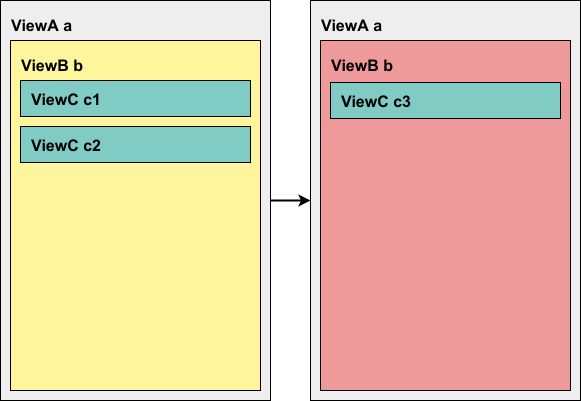
\includegraphics[width=0.8\columnwidth]{declarative_ui_example}
    \caption{Vergleich deklaratives \& imperatives UI}
\end{figure}

Im imperativen Stil würde man eine Instanz \textit{b} des so
genannten \textit{Owners} der View \textit{ViewB} nutzen
und mit Hilfe eine Selektors wie beispielsweise \textit{findViewById}
Änderungen auf dieser anwenden (und somit diese implizit invalidieren).
Das kann ungefähr so aussehen:

\begin{figure}[H]
    \centering
    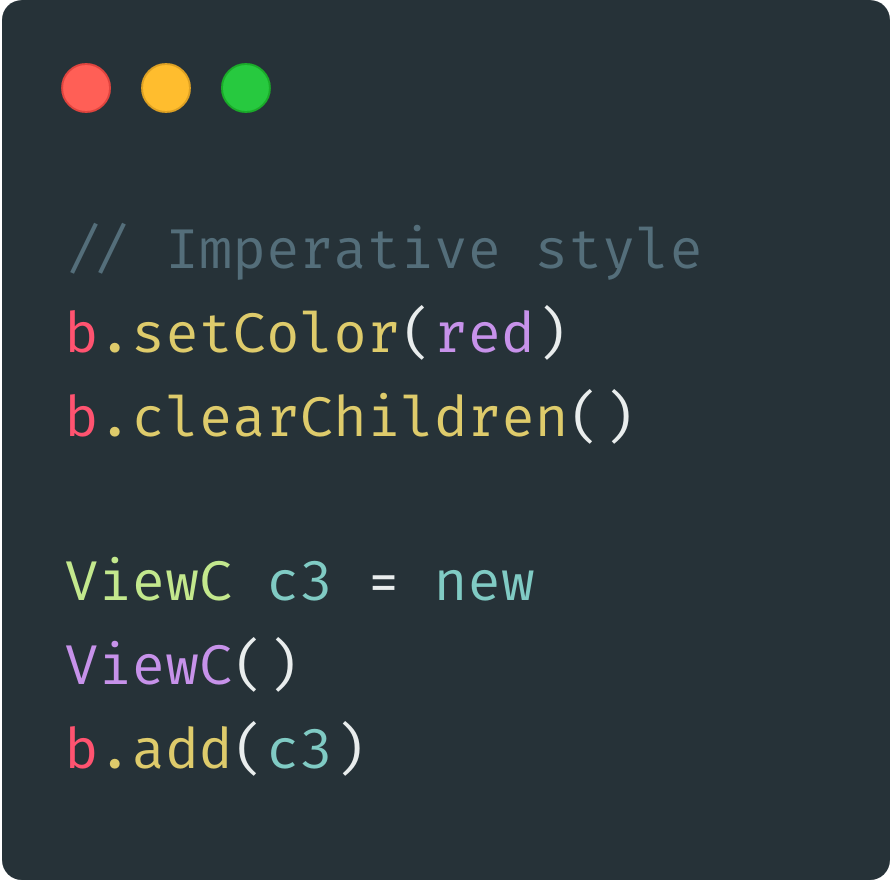
\includegraphics[width=0.4\columnwidth]{imperative_style}
    \caption{Beispiel: imperativer Stil}
\end{figure}

Außerdem müsste dieses Setup im Konstruktor von \textit{ViewB} dupliziert
werden, da die UI (der \ac{SPOT}) möglicherweise die Instanz \textit{b} überlebt.
Im deklarativen Frameworks sind View-Konfigurationen
(wie \textit{Flutter's} Widgets) unveränderlich (immutable) und an sich
nur simple Blaupausen. Um ein UI zu ändern, löst ein Widget einen Rebuild
auf sich selbst aus (in \textit{StatefulWidgets} häufig per \textit{setState()}
und erzeugt damit einen neuen Widget-Subtree.

\begin{figure}[H]
    \centering
    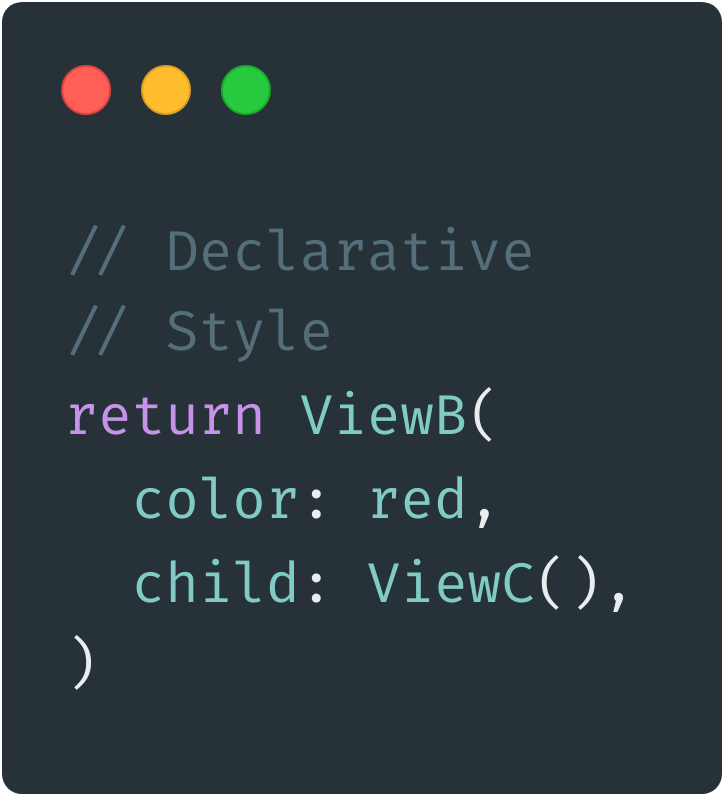
\includegraphics[width=0.4\columnwidth]{declarative_style}
    \caption{Beispiel: deklarativer Stil}
\end{figure}



\subsection{Herausforderungen}
\subsubsection{Date-Library}

\subsection{Widgets}
\subsubsection{PizzaItem}

\section{Fazit}

Die Entwicklung einer App mit \textit{Flutter}
brachte eine steile Lernkurve mit sich und bot
eine neue Sicht auf bereits bekannte Konzepte.
Als besonders herausfordernd stellte sich die
Einarbeitung und Umsetzung von Layout und Design
heraus. Auch das verhältnismäßig junge Alter
des Frameworks brachte Herausforderungen mit sich;
nicht immer gibt es aus anderen Frameworks bekannte
Bibliotheken oder entsprechende Tutorials oder
Blogbeiträge um sich Wissen neben der üblichen
Dokumentation anzueignen. In diesem Projekt nicht
betrachtet wurde die Cross-Plattform-Funktionalität
mit der auch \textit{iOS}-Apps entwickelt werden können.
Alles in allem war dieses Projekt,
auch wenn mit einem zwinkernden Auge zu sehen,
sehr lehrreich und spaßig umzusetzen.

\newpage

% Don't use page-numbers from here on
% \pagenumbering{gobble}
% \raggedright
\begin{thebibliography}{xxxxxxxxxxxxxxxxxxxxxxxxxxxxxxxxxxxx}
    \bibitem
        [Steve Krug, 2014]
        {bmbf} Don't Make Me Think! Revisited - Das intuitive Web
    \bibitem
        [Jens Jacobsen, Lorena Meyer, 2017]
        {bmbf} Praxisbuch Usability und UX: Was jeder wissen sollte,
        der Websites und Apps entwickelt - bewährte Methoden praxisnah erklärt
    \bibitem
        [Google, 2018]
        {bmbf} Angular,
        verfügbar unter: \url{https://angular.io/}\\

        Material Design,
        verfügbar unter: \url{https://material.io/design/}\\

        Material Design Components Web,
        verfügbar unter: \url{https://material.io/develop/web/}
    \bibitem
        [Dominic Carretto, 2018]
        {bmbf} Material Design Components for Angular,
        verfügbar unter:\\ \url{https://trimox.github.io/angular-mdc-web/#/home}
    \bibitem
        [Tony Spegel, 2018]
        {bmbf} Free-Rooms-Py,
        verfügbar unter:\\ \url{https://github.com/TonySpegel/free-rooms-py}\\

        Free-Rooms 2.0 "Snegon",
        verfügbar unter: \url{https://github.com/TonySpegel/Snegon}
\end{thebibliography}


\end{document}
